%%%%%%%%%%%%%%%%%%%%%%%%%%%%%%%%%%%%%%
% TRB Poster 2015
% Created by Subasish Das
% January 2015
%%%%%%%%%%%%%%%%%%%%%%%%%%%%%%%%%%%%%%

\documentclass[final]{beamer}
\usepackage[scale=1.24]{beamerposter}
\usepackage{graphicx}			% allows us to import images

%-----------------------------------------------------------
% Custom commands that I use frequently
%-----------------------------------------------------------

\newcommand{\bb}[1]{\mathbb{#1}}
\newcommand{\cl}[1]{\mathcal{#1}}
\newcommand{\fA}{\mathfrak{A}}
\newcommand{\fB}{\mathfrak{B}}
\newcommand{\Tr}{{\rm Tr}}
\newtheorem{thm}{Theorem}

%-----------------------------------------------------------
% Define the column width and poster size
%-----------------------------------------------------------

\newlength{\sepwid}
\newlength{\onecolwid}
\newlength{\twocolwid}
\setlength{\paperwidth}{48in}
\setlength{\paperheight}{36in}
\setlength{\sepwid}{0.024\paperwidth}
\setlength{\onecolwid}{0.22\paperwidth}
\setlength{\twocolwid}{0.464\paperwidth}
\setlength{\topmargin}{-0.5in}
\usetheme{confposter}
\usepackage{exscale}

%-----------------------------------------------------------
% The next part fixes a problem with figure numbering. Thanks Nishan!
%-----------------------------------------------------------

\usecaptiontemplate{
\small
\structure{\insertcaptionname~\insertcaptionnumber:}
\insertcaption}

%-----------------------------------------------------------
% Define colours (see beamerthemeconfposter.sty to change these colour definitions)
%-----------------------------------------------------------

\setbeamercolor{block title}{fg=Red,bg=white}
\setbeamercolor{block body}{fg=Black,bg=white}
\setbeamercolor{block alerted title}{fg=white,bg=Violet!70}
\setbeamercolor{block alerted body}{fg=black,bg=Maroon!10}

%-----------------------------------------------------------
% Name and authors of poster/paper/research
%-----------------------------------------------------------

\title{Lane Conversion for Urban Roadway: An Unideal but Effective Way to Improve Roadway}
\author{Xiaoduan Sun, PhD \& PE, Professor \hspace{5in} Subasish Das, PhD Candidate}
\institute{University of Louisiana \hspace{10in} University of Louisiana }

%-----------------------------------------------------------
% Start the poster itself
%-----------------------------------------------------------


\begin{document}
\begin{frame}[t]
  \begin{columns}[t]												% the [t] option aligns the column's content at the top
    \begin{column}{\sepwid}\end{column}			% empty spacer column
    \begin{column}{\onecolwid}
      \begin{alertblock}{Research Question}
        {\rmfamily{Is inexpensive countermeasure like lane conversion for urban roadway effective?}}
      \end{alertblock}
      \vskip2ex
      \begin{figure}
              \begin{center}
                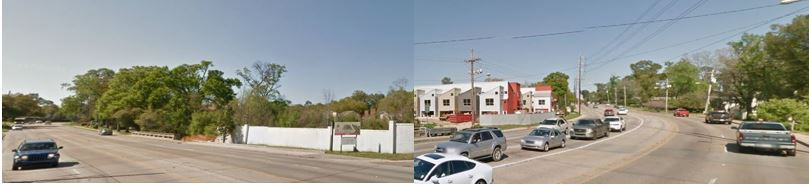
\includegraphics[width=10.5in, height= 3in]{as3.jpg}

              \end{center}
      \end{figure}
      \begin{block}{Abstract}
        {\rmfamily{Undivided roadways have consistently exhibited low safety performance, particularly in urban or suburban areas where roadside development is relatively intense. This study introduces a low cost crash countermeasure successfully implemented on four different segments of undivided roadways in Louisiana. This crash countermeasure is to change an undivided four-lane roadway to a five-lane roadway with a center lane for left turns by restriping pavement markings without increasing pavement width. Based on the statistical analysis, the crash modification factors for all roadways are estimated to be less than 0.6 with a standard deviation less than 0.07. Although it is not surprising to see the biggest crash reduction comes from the rear-end collisions, the other types of collision are also reduced.}}
      \end{block}
      \vskip2ex

      \begin{block}{Background}
        {\rmfamily{In Louisiana, there are 1,530 miles of undivided multilane roadways, and most of them are four-lane highways on the Louisiana Department of Transportation and Development System (LaDOTD). With sufficient pavement width, a four-lane undivided highway can also be easily changed to a five-lane roadway with the center lane for left turns, which expectedly reduces rear-end collisions. This option, even though it is the least expensive one, is less desirable based on past experiences with five-lane roadway operations in many urban and suburban areas which is reexamined in this study.}}
      \end{block}
    \end{column}

   \begin{column}{\sepwid}\end{column}			% empty spacer column
    \begin{column}{\twocolwid}							% create a two-column-wide column and then we will split it up later
      \begin{columns}[t,totalwidth=\twocolwid]	% split up that two-column-wide column

        \begin{column}{\onecolwid}\vspace{-.69in}
          \begin{block}{Site Selection}
            \begin{figure}
              \begin{center}
                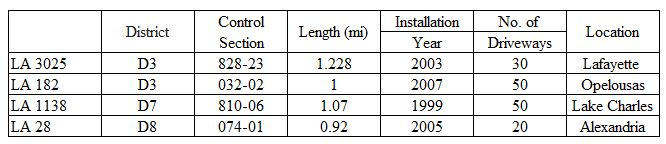
\includegraphics[width=11.2in, height=2.5in]{as4.jpg}

              \end{center}
            \end{figure}
          \end{block}
        \end{column}
        \begin{column}{\onecolwid}\vspace{-.69in}
                  \begin{block}{Crash Reduction Summary}
            \begin{figure}
              \begin{center}
                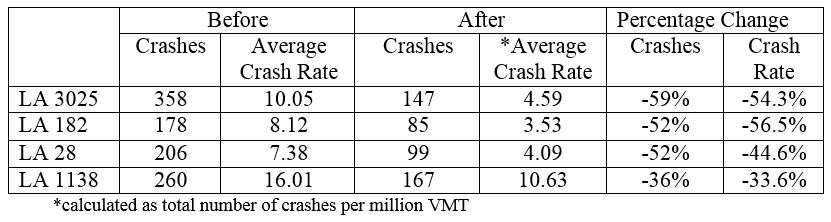
\includegraphics[width=11.2in, height=2.8in]{as5.jpg}

              \end{center}
            \end{figure}
            \end{block}
        \end{column}

\end{columns}
      \vskip2ex
      \begin{alertblock}{\textbf{Study Sites}}		% an ACTUAL two-column-wide column
            \begin{figure}
              \begin{center}
                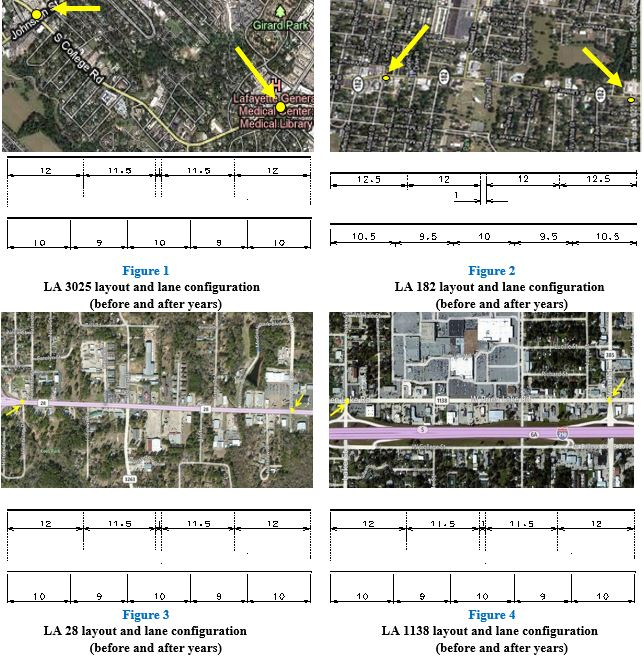
\includegraphics[width=17in, height= 13in]{ac3.jpg}

              \end{center}
            \end{figure}
      \end{alertblock}
        \vskip2ex

        \begin{columns}[t,totalwidth=\twocolwid]	% split up that two-column-wide column
        \begin{column}{\onecolwid}\vspace{-.69in}
          \begin{block}{Methodology}
             {\rmfamily{In this study, \textbf{four-step} procedure introduced by Dr. Ezra Hauer was used to estimate the CMF.  }}\\
               \vspace{0.25in}
             \begin{figure}
              \begin{center}
                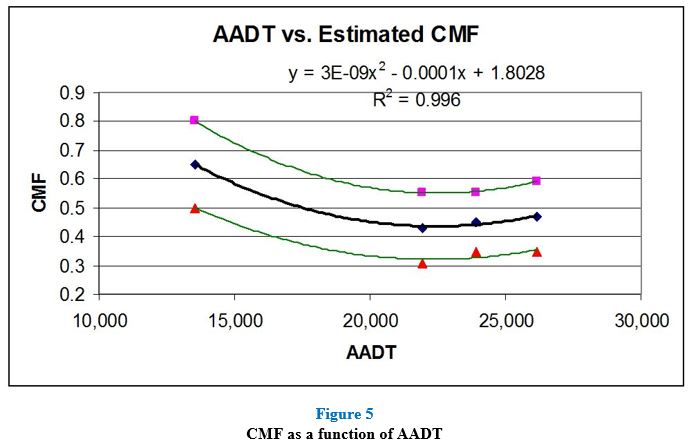
\includegraphics[width=10.5in, height= 5in]{azz3.jpg}
                %\caption{CMF as a function of AADT.}
                %\label{fig:multDom}
              \end{center}
            \end{figure}

          \end{block}
        \end{column}
        \begin{column}{\onecolwid}\vspace{-.69in}
                  \begin{block}{Crash Modification Factor}
            {\rmfamily{The estimated expected CMF is 0.45, 0.43, 0.47 and 0.65 for these four roadway segments respectively. The corresponding standard deviations are 0.051, 0.062, 0.062 and 0.075.  }}\\
            \vspace{0.25in}

         \begin{figure}
              \begin{center}
                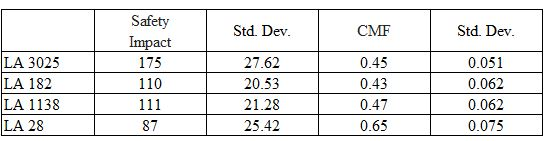
\includegraphics[width=10.5in, height= 2.5in]{as7.jpg}

              \end{center}
            \end{figure}


          \end{block}
        \end{column}
        \end{columns}


\end{column}

  \begin{column}{\sepwid}\end{column}			% empty spacer column
  \begin{column}{\onecolwid}
    \begin{block}{Crash Characteristics}
            \begin{figure}
              \begin{center}
                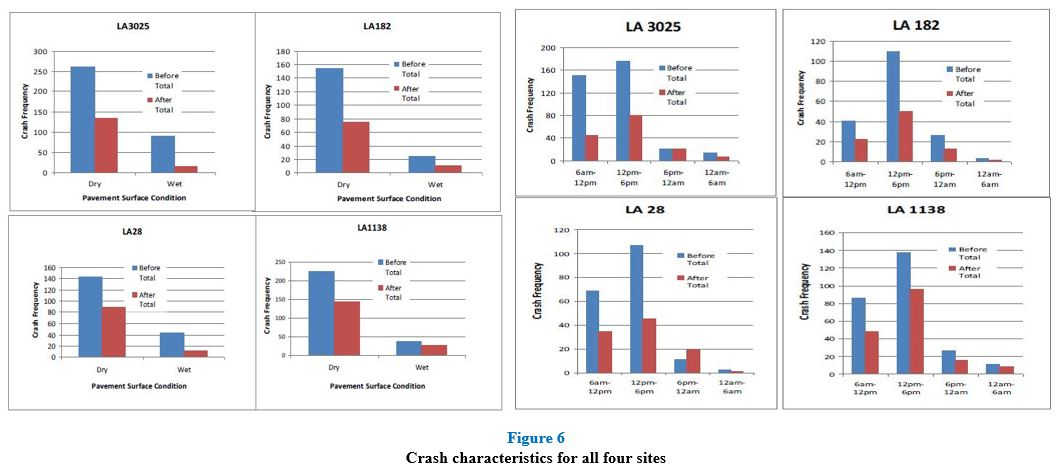
\includegraphics[width=10.8in, height= 5 in]{azz1.jpg}

              \end{center}
            \end{figure}
    \end{block}
    \vskip2ex


        \begin{block}{Benefit-Cost Analysis}
            \begin{figure}
              \begin{center}
                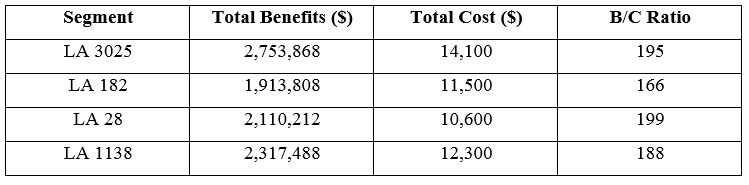
\includegraphics[width=10.5in, height=2.5in]{ad3.jpg}

              \end{center}
            \end{figure}
        \end{block}
    \vskip2ex

        \begin{block}{Conclusions}
            {\rmfamily{Examining these two successful crash reduction cases, it is important to note that onesize-fits-all solutions do not always prevail in highway safety. Although this study shows impressive results, caution must be taken when applying this crash countermeasure in other locations. Particular attention must be made to not only the number of driveways but also the type and size of traffic generators along the roadway and existence of other travel modes.With sufficient segments (samples), it would be interesting to investigate whether the presence and size of retail business make a difference in the magnitude of the CMF. Also noted that both roadway segments are not major bus corridors and do not have noticeable bicycle and heavy truck traffic, which makes the lane conversion possible.}}\\
    \vskip2ex

      \begin{center}
        \begin{tabular}{ccc}
          
\includegraphics[width=3in, height= 3in]{ulls.jpg} & \hspace{1.25in} & 
\includegraphics[width=3in, height=3in]{ltrc.jpg}
        \end{tabular}
      \end{center}
    \end{block}
  \end{column}
  \begin{column}{\sepwid}\end{column}			% empty spacer column
 \end{columns}
\end{frame}
\end{document}
